\chapter{开发问题记录}

\section{开发技巧}   

\subsection{Qt包含目录}
在使用Qt的某一个模块的时候,需要include相应的头文件,为了告诉编译器头文件的具体位置,需要在pro文件中指定需要使用的相关模块,这样qmake会对pro文件进行处理,生成相应的路径。也可以指定不是用某些库。

常见的模块有:core、gui、widgets等,如果想要包含private的头文件,那么就需要接着添加core-private、gui-private、widgets-private等。具体的效果可以使用VS打开pro文件,然后查看相应的头文件设置信息。          

\subsection{预编译文件}
当一个工程项目很大时,会出现很多的头文件,这个时候,把他们全部一次性加入到工程当中是一件非常繁琐和头疼的事情。在Qt当中,可以进行这样的方便设置。将每一个模块的代码(包括h文件和cpp文件)单独放置在一个文件下面,然后再新建一个pri文件,在pri文件当中设置需要include的文件列表。这样,当我们需要使用这个模块时,不需要再把源代码加入到工程当中,只需要把该pri文件include到pro文件当中,这样就可以了。

\subsection{Qtcreator子项目}
在一个较大的工程项目当中,会有多个子项目,同时编译得到最后的文件。这在vs当中被称为solution。qtcreator当中也有类似的功能。

主要的操作是:在顶部的pro文件当中设置模板TEMPLATE为subdirs模式;然后设置SUBDIRS,添加指定的工程模块;使用"CONFIG+=ordered"配置为顺序编译。需要注意的是每一个单独的子项目都需要能够单独编译成功。为了方便,可以将这些工程的目标文件的生成路径设为一致。

这个子项目跟上面的pri文件不同,该文件对应的是一个项目很多时,包含很多模块进行简化。

\subsection{default构造函数}
在C++当中,类里面的数据大部分都是私有的,外部无法访问的,所以需要定义一些函数来进行赋值或者初始化的操作,这些函数可以称为接口。C++的类通过构造函数来对数据进行初始化操作,一个类当中可以有多个构造函数,这些函数的名称跟类名一致。当在类中没有定义任何构造函数时,C++会给你提供一个无参数的默认构造函数。但是,当你定义了一个含有参数的构造函数时,编译器就不再提供这个构造函数,如果你需要使用这个函数,就需要自己自已一个,否则,编译器就会报错。为了减轻程序员的负担,在C++的类声明时,使用"=default"来表示让编译器生成一个默认的构造函数,这样就不需要自己再去实现了。这个构造函数是在类的内部实现的,所以是一个内联函数。但是,vs2013之前的编译器都不支持这种语法,会报错。

需要注意的是,在vs2013当中遇到了这个错误:multiple versions of a defaulted special member functions are not allowed。原因可能是,使用default定义了一个默认构造函数,同时定义了一个含有参数的构造参数,但是这个参数的默认值被设为了null,编译器就认为出现了两个默认构造函数,所以会报错。

\subsection{error LNK2019: unresolved external symbol compress referenced in function}
如果使用Qtcreator出现了这个问题,恰好编译器是vs的话,有可能是一下原因:确定一下在pro文件当中,头文件列表和源文件列表中被调用函数的源文件是不是出现在了调用文件的后面,如果是的话,将它移动到前面去。

\subsection{构造函数}
1.父类没有声明构造函数

(1)子类也没有声明构造函数,则父类和子类均由编译器生成默认的构造函数;

(2)子类中声明了构造函数(无参或者带参),则子类的构造函数可以写成任何形式,不用顾忌父类的构造函数。在创建子类对象时,需要先调用父类的默认构造函数(编译器自动生成),然后再调用子类的构造函数。

2.父类只声明了无参数构造函数

如果子类的构造函数没有明显地调用父类的构造函数,则将会调用父类的无参构造函数。

3.父类只声明了带参数的构造函数

子类的构造函数必须显式得调用父类的构造函数。

4.父类同时声明了无参和有参构造函数

子类的构造函数调用其中一个即可。如果没有显式调用的话,会默认调用父类无参构造函数。

\subsection{Texstudio与sumatrapdf反向搜索关联}

sumatrapdf是一款免费小巧的PDF阅读器,双击PDF的某一个区域,可以打开关联的tex文件的相应位置。对于winedit,"D:/My Program Files/CTEX/WinEdt/WinEdt.exe" "[Open(|\%f|);SelPar(\%l,8)]"
对于TeXstudio"D:/My Program Files/TeXstudio/texstudio.exe"  "\%f" -line \%l

\subsection{VS不同版本编译报错}
出现“无法找到文件MSVCP120D.DLL”的问题,问题在于某些使用的dll文件是vs2013生成的,而现在使用的vs版本不是2013,解决方法就是将这些dll在新的vs下重新编译。

\subsection{Qt国际化}
在软件当中,需要实现界面的中文显示,这里采用的是Qt的国际化方案,也就是提供针对软件界面文字的中国版本的翻译文件,将国家设为中国就可以了。

简单介绍一下实现的步骤(详细的可以参考网上的教程):首先,在你需要翻译的地方,字符串需要写在tr函数当中,然后在pro文件当中加入ts文件,接着运行lupdate命令,生成相应的ts文件;然后使用语言家软件打开ts文件,或者你直接打开ts文件进行编辑,设置好相应的翻译;完成之后,运行lrelease命令生成压缩版的翻译文件qm;然后就是怎么使用的问题了,网上有好几种方案,一种就是放在exe文件的运行目录,另一种就是将qm文件放到工程的资源文件当中,这样的好处就是避免了文件的丢失,别人的篡改等等,可以编译进二进制文件当中。而且,如果加入到资源文件当中,每次自动生成qm文件就还在那个位置,就不需要你把它再拷贝到exe目录里。

简单说一下,在load qm文件时遇到的坑。我已经把qm文件加入到了qrc文件当中,但是无论如何都不能正确的载入,网上搜索了各种教程也不行。qm文件其实也拷贝到了文件夹下,也是不行。后来在res文件夹下面新建了一个translations文件夹,然后qm文件都放在了里面,然后接着load就好使了,我也不知道是为什么。

需要注意的是,如果在不同分支当中同时运行了lupdate来更新翻译,由于ts文件会继续翻译短语的所在文件和行号,所以合并的时候,ts文件可能会出现冲突。可以采用一个不生产行号的方法来折中处理。但是为了避免麻烦,还是在单一的分支当中提交翻译吧。

\subsection{如何保存程序的配置信息?}
在程序的运行过程当中,用户可能会对窗口的位置、大小进行一些改变,或者程序的一些信息做了更改,如何在下次启动时能够保持原样?在Qt当中,是通过配置文件实现的。

\subsection{如何在状态栏上添加一些复杂的控件?}

\subsection{warning: C4819: The file contains a character that cannot}
你的源码是不带BOM的UTF8格式,但是MSVC不知道你用的UTF8。由于你在简体中文Windows系统下,它就认为你用的是GB18030(也叫GB2312,GBK,CP936)。

当你一个汉字时,占3个字节,用GB18030是无法解析的(1个半汉字)。当你2个汉字时,占6个字节,用GB18030碰巧可以解释成3个汉字。

如果不指定的话默认是 utf-8。所以我们用 gcc 时很少关注这个问题。

Viual Stdio 中就麻烦多了。这里先说 Visual stdio 2015,这个是我现在用的编译环境。VS2015 中如果源代码是 utf-8的,执行字符集默认是本地 Locale 字符集,对于简体中文的 windows 系统来说,这个 本地Locale字符集是 gb18030。所以直接显示汉字会全是乱码。解决这个乱码有三个办法,第一个办法是编译时加入命令行参数,在 Qt 的 pro 文件中可以这样:

msvc:QMAKE\_CXXFLAGS += -execution-charset:utf-8
1
第二个办法是在源文件中加入:

\#pragma execution\_character\_set("utf-8")

\subsection{如何制作图标?}
SVG格式的图标怎么制作?适用于什么情况?

\subsection{生成注释}
为了方便阅读源代码,需要自动生成注释。从源代码当中提取注释并生成文档的方案是有的,那就是doxygen,但是一个个去添加固定格式的注释简直很烦诶,还需要自动根据代码当中的函数添加注释模版。这个东西貌似需要IDE支持。

1.doxygen的安装

如果IDE是qtcreator的话,可以安装doxygen的插件,直接去\href{https://github.com/fpoussin/qtcreator-doxygen}{Github qtcreator-doxygen}下载。这个插件的编译需要跟qtcreator的源代码一起编译生成,所以你必须下载对应版本的插件,其实就是一个dll文件。

下载好dll文件后,将其放到qtcreator安装目录下的plugins目录,然后重启就可以了。之后,就会在工具菜单下多了一个doxygen子菜单,然后就可以自动地给整个文件添加注释了。这个注释最好添加在源文件当中。

添加完注释之后,就是利用doxygen生成文档了。

2.doxygen的编译

网上仅提供了某些版本的二进制文件,但是没有最新版,如何编译得到最新版qtcreator的doxygen插件?

\subsection{Paint事件}
导致画面闪烁的关键原因分析:

一、绘制窗口由于大小位置状态改变进行重绘操作时,绘图窗口内容或大小每改变一次,都要调用Paint事件进行重绘操作,该操作会使画面重新刷新一次以维持窗口正常显示。刷新过程中会导致所有图元重新绘制,而各个图元的重绘操作并不会导致Paint事件发生,因此窗口的每一次刷新只会调用Paint事件一次。窗口刷新一次的过程中,每一个图元的重绘都会立即显示到窗口,因此整个窗口中,只要是图元所在的位置,都在刷新,而刷新的时间是有差别的,闪烁现象自然会出现。所以说,此时导致窗口闪烁现象的关键因素并不在于Paint事件调用的次数多少,而在于各个图元的重绘。

根据以上分析可知,当图元数目不多时,窗口刷新的位置也不多,窗口闪烁效果并不严重;当图元数目较多时,绘图窗口进行重绘的图元数量增加,绘图窗口每一次刷新都会导致较多的图元重新绘制,窗口的较多位置都在刷新,闪烁现象自然就会越来越严重。特别是图元比较大绘制时间比较长时,闪烁问题会更加严重,因为时间延迟会更长。
解决上述问题的关键在于:窗口刷新一次的过程中,让所有图元同时显示到窗口。

二、进行鼠标跟踪绘制操作或者对图元进行变形操作时,当进行鼠标跟踪绘制操作或者对图元进行变形操作时,Paint事件会频繁发生,这会使窗口的刷新次数大大增加。虽然窗口刷新一次的过程中所有图元同时显示到窗口,但也会有时间延迟,因为此时窗口刷新的时间间隔远小于图元每一次显示到窗口所用的时间。因此闪烁现象并不能完全消除!所以说,此时导致窗口闪烁现象的关键因素在于Paint事件发生的次数多少。
解决此问题的关键在于:设置窗体或控件的几个关键属性。

解决双缓冲的关键技术:

1、设置显示图元控件的几个属性: 必须要设置,否则效果不是很明显!
this.SetStyle(ControlStyles.OptimizedDoubleBuffer | ControlStyles.ResizeRedraw |ControlStyles.AllPaintingInWmPaint, true);

2、窗口刷新一次的过程中,让所有图元同时显示到窗口。

可以通过以下几种方式实现,这几种方式都涉及到Graphics对象的创建方式。
Graphics对象的创建方式:

a、在内存上创建一块和显示控件相同大小的画布,在这块画布上创建Graphics对象。接着所有的图元都在这块画布上绘制,绘制完成以后再使用该画布覆盖显示控件的背景,从而达到“显示一次仅刷新一次”的效果!

b、直接在内存上创建Graphics对象:

\subsection{MSVC中文注释导致的编译错误}
遇到这个问题是将代码在虚拟机下面进行编译的时候出现的。在另外一台电脑上编译运行没有任何问题,但是在这台电脑上运行就好几百个问题,刚开始也是丈二和尚,后来慢慢领悟到应该又是中文编码的问题导致没有正确的解析源代码。

为什么会出现编码错误呢?主要是中文的存在。编码主要存在在两个地方:一个是IDE需要知道文件的编码来正确地进行源代码的显示;第二个就是编译器需要知道文件的编码来正确地对代码进行编译。我们所遇到的错误就是第二个导致的。这个问题的根源在于MSVC编译器对UTF-8编码支持的不是很好。简单来说,就是在Windows下,微软创建的UTF-8文件都自带BOM,而UNIX系的UTF-8文件则不带。MSVC编译器则是通过判断文件有没有BOM来确定是不是要采用UTF-8编码,所以Unix下的UTF-8编码文件拷贝到Windows下使用MSVC进行编译就会不通过。没有BOM,编译器就会采用操作系统的本地语言编码进行解释,中文应该是GB2321。这就很愚蠢了。

解决办法主要有以下几种:
\begin{enumerate}
	\item 将所有的UTF-8文件都加上BOM。这个方法虽然可行,但是不适合跨平台,而且BOM有可能在别的地方打开之后被删掉。还有那么多文件都要批量添加BOM。
	\item 所有文件的编码都改为UTF-8,注释一律用英文。经测试,这个方法可行,没有报错。但是不支持中文注释也太傻逼了吧,都什么年代了。
	\item 所有的文件编码依然采用UTF-8,这样可以跨平台,但是想办法让编译器忽略掉中文注释。注释本来就是被编译器忽略的一部分,但是因为解码错误,编译器只能识别出注释的开始部分,也就是"//"。但是后面的中文如果识别不出来的话,就会连带注释后面的英文代码也变成了注释,直到解析出了换行。所以解决办法就是让编译器识别出注释的结束,想来想去,只有多行注释这种方法了,也就是“/**nnnn**/”。经实测,这种方法可行,但是就是得两个星号。
\end{enumerate}

详细的解释可以参考:\url{https://blog.csdn.net/imxiangzi/article/details/50781459}、 \url{https://www.cnblogs.com/Esfog/p/MSVC_UTF8_CHARSET_HANDLE.html}、 \url{https://www.cnblogs.com/cheungxiongwei/p/8003867.html}、 \url{https://blog.csdn.net/liyuanbhu/article/details/72596952}。

\subsection{只安装MSVC编译器}
在虚拟机当中进行代码的测试,但是发现VS的安装文件实在太大了,萌生了只安装编译器的想法,因为自己也不使用别的东西。在网上搜索了一下,真有相关的资料。

\subsection{Qt的元对象系统}

\subsection{Qt QFlags}

\subsection{error: LNK2019: unresolved external symbol referenced in function}

明明没有什么问题的项目编译之后却报这个错误,开始的时候确实令人匪夷所思。在另外一台电脑上编译运行也没有什么问题。解决办法就是将build目录删除,然后重新编译运行,就没有这个错误了。

\subsection{面向对象的类的设计}

\subsection{不同的上下文的动作实现}
在软件当中,通常要实现这样的操作,比如主窗口内有很多的控件,每一个控件可能都有自己对应的复制粘贴删除的动作,按下相应的快捷键之后,如何判断现在是属于哪个控件,应该执行哪个控件对应的命令。

我按下del键,有可能是删除文件,也有可能是删除图形,如何进行相应的判断?

\subsection{工程树当中的数据保存问题}
在Qt当中,树形控件是采用视图模型委托的设计模式,也就是,你需要自定义对应的抽象类文件,实现子类。Qt已经实现好了数据读取,设置的函数模版,你只需要重新根据你的需要进行实现即可。自由度最大的就是真实数据的保存,很明显,传递给树控件的数据和真实的数据还是应该分离的。那么真实的数据应该保存在什么位置?project的类变量当中?毕竟这是属于这个项目的。那么新的问题就来了,需要更多的新的数据类型,比如你要自定义变量类型吧,然后你在project当中保存一个变量的list或者map。你还要实现材料,几何,分网,还有一堆杂七杂八的东西。你需要监控这些变量的改变,然后对应的更新树控件当中的node显示,反过来也是一样的,如果对node进行了相应的修改操作,那么就需要更新对应的变量。问题是,采用什么样的方法进行更新呢?应该是在修改后直接更新吧。

如何将node的数据与真实的数据关联起来?
\subsection{Node的设计问题}
工程树当中有很多的node,不光是数量多,而且种类也非常的多。应该如何设计它的继承关系?比较纠结的就是一个node类型目前设置的是没有子节点的,所以它应该是直接从顶层node继承过来的,如果以后想要更改功能,给它添加子节点,那就要再次修改它的继承关系啊。
\subsection{动作的管理}
在一个大型的软件当中,必然会有数不清的actions,而且在一个类当中可能要去调用另外一个类的action,所以就需要一种策略来将所有的actions集中存储起来。集中存储的话避免不了前面说的一个问题,相同的动作ID。

现在知道了应该创建一个map或者hash类型的变量来保存变量,并实现检索。hash的好处就是搜索速度能够快点儿。但是,由于现在采用的不是菜单风格,ribbon式的UI它不光可以添加action,它还可以添加widget,这样留出接口就比较麻烦了吧。
\subsection{材料树}
材料树跟工程树不太一样,因为里面只包含材料,多一点的可能就是材料的分类,这个就相当于是一个容器或者文件夹。

有一种想法,材料的确是一个大类,非常复杂,但是,当我们去查询某个材料的某个属性的时候,就像是查询数据库一样的,它有那个材料属性的名字,然后对应的有一个单位和数值。所以,想要将材料设计的更加丰富,可以将其抽象为属性的集合,这些属性从属于不同的分类和学科,也有可能只存在于某些条件下,只在特定的情形才会有这个属性。这样的设计,材料可简单,可复杂。其实,在设计软件的时候,并不是不能找到一种解决方案,而是,太不容易开始,又太容易考虑太多的未来的东西而缚手缚脚。你写得东西要给别人用,要一直用,要给更多的模块用,
\subsection{代数模块}
需要很好的定义一些代数模型,并保证不随便更改。包含矩阵,向量,线性操作。当然要注重性能和实用性。稳妥的方式就是采用现成的模块。
\subsection{常量引用}
在C++当中,函数的参数是以形参的形式传递的,也就是,编译器会将原始的数据拷贝一份,放到另外一个地方供你使用,你对该变量的任何修改都不能使原始数据发生变化。所以,起初C当中是采用指针的方式传递真实的地址来实现对原始数据的修改。在C++当中,引入了引用类型,该类型相当于是原始数据的一个别名,但是可以达到修改真实数据的目的。在阅读别人的源代码时,发现在函数的参数当中,传递的大多都是const类型的引用,仔细一思考,这就很矛盾。引用类型是用来修改数据的,加了一个const限制又代表不让修改,那么为什么这样写呢?这是为了提高程序的性能。由于在C++当中,是采用创建临时对象的方式传值的,所以编译器会创建一个拷贝,这样的话就需要调用构造函数和析构函数,消耗额外的计算和存储资源。
\subsection{上下文}
上下文到底意味着什么?
\subsection{变量和函数何时应该声明为static}
static变量具有全局的属性,使用类名就可以直接访问,生命周期也比其他变量要长。那么static变量的空间受不受到什么限制?可以无限分配吗?

在类中声明static变量或者函数时,初始化时使用作用域运算符来标明它所属类,因此,静态数据成员是类的成员,而不是对象的成员,这样就出现以下作用:

(1)类的静态成员函数是属于整个类而非类的对象,所以它没有this指针,这就导致 了它仅能访问类的静态数据和静态成员函数。      

(2)不能将静态成员函数定义为虚函数。      

(3)由于静态成员声明于类中,操作于其外,所以对其取地址操作,就多少有些特殊 ,变量地址是指向其数据类型的指针 ,函数地址类型是一个“nonmember函数指针”。

(4)由于静态成员函数没有this指针,所以就差不多等同于nonmember函数,结果就 产生了一个意想不到的好处:成为一个callback函数,使得我们得以将C++和C-based X W indow系统结合,同时也成功的应用于线程函数身上。 (这条没遇见过)  

(5)static并没有增加程序的时空开销,相反她还缩短了子类对父类静态成员的访问 时间,节省了子类的内存空间。      

(6)静态数据成员在<定义或说明>时前面加关键字static。      

(7)静态数据成员是静态存储的,所以必须对它进行初始化。 (程序员手动初始化,否则编译时一般不会报错,但是在Link时会报错误) 

(8)静态成员初始化与一般数据成员初始化不同:

初始化在类体外进行,而前面不加static,以免与一般静态变量或对象相混淆;

初始化时不加该成员的访问权限控制符private,public等;     
   
初始化时使用作用域运算符来标明它所属类;

所以我们得出静态数据成员初始化的格式:

<数据类型><类名>::<静态数据成员名>=<值>

(9)为了防止父类的影响,可以在子类定义一个与父类相同的静态变量,以屏蔽父类的影响。这里有一点需要注意:我们说静态成员为父类和子类共享,但我们有重复定义了静态成员,这会不会引起错误呢?不会,我们的编译器采用了一种绝妙的手法:name-mangling 用以生成唯一的标志。
\subsection{项目文件保存需要注意什么}
随时都会对项目树进行操作,就会产生新的数据,需要立即保存吗?保存的话可能是在文件中插入,是重新保存一次吗?
\subsection{signals 和 slots}
这两个东西我都理解是什么 ,但是有一个问题,什么时候需要自定义signals?
\subsection{如何测试?}
有数不清的函数和类文件,大多数有很大的依赖性,如何脱离项目完成单独的测试?
\subsection{初始化列表}
C++的构造函数的初始化有两种方式,一种是初始化列表,一种是在构造函数内部执行。第一种的话,只会初始化一次,而第二种在执行之前,会先调用父类的构造函数进行初始化。
\subsection{vs2017 char *}
在新版本的vs2017当中,向函数参数传递常量字符串的时候,会无法转换的错误。这个错误产生的原因似乎是由于在C++11的标准中,不能直接将常量赋值给指针变量,解决办法就是在常量字符串前面加上指针的强制转化符。
\subsection{qflags}
在软件当中,有的时候就会有很多的标志作为判断,比如保存图形有没有被选中,是不是可见,等等,需要一个变量来保存状态,如果每一个都采用单独的变量,那么肯定非常的浪费空间,最合力的方法还是用bit位操作进行。Qt当中有一个QFlag的类,专门用来

QFlags的本质
QFlags(通常称为标志)是Qt中内置的模板类,其主要作用是为枚举值及其组合运算提供类型安全的算法。比如有如下枚举
enum E{a=1, b=2, c=3};
则void f(E);可接受枚举类型E的成员值,但是不能接受其组合运算的值,比如f(a|b);是错误的,因为a|b的结果是int型而不是类型E。若把函数声明为void f(int);则可以接受枚举值的组合运算,但是同时还能接受整型等其他类型,这是类型不安全的行为。
QFlags类就是为了解决以上问题的,比如f(QFlags< E>); 则f就只能接受类型为E的成员值的组合运算。由此可见,QFlags通常与枚举类型是一起使用的。
在Qt中通常把标志使用typedef进行重新命名(因为QFlags是模板类其类型名太长),重命名之后的名字与对应的枚举类型名字通常只在末尾相差一个字母s,比如与枚举类型E对应的标志通常被重命名为Es,其语法为typedef QFlags< E> Es;
综上所述,在Qt中,若函数的形参是标志,则实参可以是多个按位“或”的枚举类型值,若函数的参数是枚举,则只能指定该枚举类型的单个值,不能使用按位“或”运算符。

\subsection{初始化列表和构造函数内赋值}
对于内部数据类型,一般都比较简单,这两种方法的计算效率没有多大的差异;

如果没有采用初始化列表,那么在函数内部就会调用父类的默认构造函数对父类的变量进行初始化,如果父类没有提供默认的无参数的构造函数,那么就会报错,这个时候你就只能在初始化列表当中调用含有参数的构造函数进行初始化了;

对于类当中的const、引用数据成员,必须在初始化列表当中进行初始化,因为在函数内部就成为了赋值;

对于类当中的类成员变量,如果在初始化列表当中初始化,相当于调用了一次拷贝函数,而在构造函数内部,就会调用一次构造函数,然后再调用一次赋值函数。这样,计算效率就下降了。

但是,如果类成员变量如果是指针的话,不就没有这个问题了?

列表初始化的顺序与声明顺序相同,因此要考虑变量之间有没有初始化的顺序问题。
\subsection{virtual析构函数}
如果一个类有可能被继承,那么它的析构函数最好加上virtual,不然会出现内存泄漏问题,找都找不到原因。
\subsection{单元测试}
单元测试好像不是我所认为的测试。
\subsection{材料}
如何定义材料类,也是一个非常值得研究的事情。因为,材料实在是太复杂了。有着数不清的属性。在某些研究当中,只有某几个属性有利用价值,其余的没有使用价值。如果定义一个包含所有属性的类,必然会浪费很多的空间。那么就应该具有添加自定义属性的功能,根据需要生成某些特征。
\subsection{qtcreator的模式}
需求分析,定制功能,任务拆解,技术支持,功能实现。设计的思维,理念,技巧,套路,模版。

以主窗口为核心,对外提供操作的接口。接口的当中提供的控件不会无故添加在主窗口当中,需要提前在这个类当中提前声明控件的指针,并提供接口。
\subsection{函数的实现}
类当中的成员函数,不一定要在对应的cpp文件当中全部实现,可以在h文件当中实现,也可以分散在好几个文件当中实现,有时候采用这种方式可能是为了调用该文件当中的某一个函数,或者要被调用。
\subsection{有限元求解的必要因素}
为了完整的求解一个有限元问题,需要那些因素?注意,是所有的,而不是一些不可缺少的,有的问题需要而有些问题不需要的。
\subsection{有限元类的设计}
所有的求解变量都应该存储在project类当中,包括几何模型、材料、物理属性、分网等等数据,因为求解当中是以project为核心的,不能将数据放置到别的地方,这样就容易被其他的项目修改。同样的,一系列的求解操作都应该放在project当中进行实现。

那么有一个问题,是projecttreewidget包含project还是project包含它?应该是比project更高的一级拥有这个东西。
\subsection{如何规定当前求解问题的类型?}
如果不设计更加具体的project子类,通过什么方法来辨别求解问题的类型,所需要的物理公式?真的能够多物理场吗?
\subsection{信号槽}
只有真实的对象之间才能产生信号槽。克服屏幕分辨率低,显示像素差的方法就是放大字号。
\subsection{菜单}
如何在系统栏添加菜单?这个操作并不是在主函数当中一次完成的(指的是插件风格的写法),每一个插件都有跟自身相关的操作菜单,所以这部分菜单的生成可以放在对应模块的初始化部分执行,这样更加具有合理性。随用随加,用完就删。但是这样的写法还没有针对ribbon风格进行测试,毕竟ribbon的api似乎没有menu那样的丰富,不知道最后的显示效果会是什么样。不知道ribbon和menu之间有没有一些转换的函数。但是ribbon比menu的高级的地方在于,ribbon当中可以放置更加复杂的widget。另外一个ribbon需要解决的就是,能不能在任意一个group之前插入,如果可以的话,就可以对照着menu进行修改了,但是还是觉得效果可能没有menu那样的优雅。
\subsection{menu与group的区别}
在一个menu当中,插入一个menu,效果就是插入了一个子菜单,但是如果插入了一个group,就是插入了一组动作,菜单列表是在一级显示的。对于菜单,可以不断地嵌套式地插入,但是,ribbonbar的widget控件就不能这样干了。
\subsection{运行当中的无效菜单如何设置?}
通常,软件当中,根据运行环境的判断,某些菜单在这个情景下可能会失效,这个效果如何才能实现。实现的原理就是添加一个信号槽,信号就是菜单将要显示,连接上更新菜单的动作即可。
\subsection{SessionManager是干嘛的}
这个貌似是一个项目管理与当前运行之间的一个接口。
\subsection{磁材料建模}
线性、非线性材料;
\subsection{导航控件}
没有写代码之前,没有研究别人的代码之前,并没有认识到自己想法的单纯和简单。也就是没有什么经验。对功能的认识不够清楚,研究地不够明澈。可以说,理解的非常的狭隘,不利于代码实现。例如,最开始对项目的认识,以为就是一个对xml文件进行读写的类,可是仔细的研究别人的写法,发现并不是这样的,或者说并不是全部。project类并不是项目插件的核心,只是一个小的模块,你不可能只是只打开一个项目,所以你要管理项目,项目还会有很多添加删除的动作。项目不光有数据,还要有控件,而这个树控件,肯定要包含一些跟项目有关的东西,所以它不能是标准的树控件,必须对他进行自定义,添加自己的数据模型。然后把这些都封装进project的模型当中,然后再把project放进项目管理器当中进行管理。项目这块儿是绝对的核心,其他的什么编辑器啊,别的都是被调用的,用来显示项目当中的数据的。最好的设计方法就是要把足够独立的模型给建立成一个类,利用类之间的包含关系,再建立更加复杂的对象模型。导航控件不只是只有树,还有其他的按钮之类的,所以应该单独地建立为新的控件。
\subsection{dockwidget}
如果在窗口当中添加了dockwidget,好像是自动带分割器的,如果就是普通的,那么就得自己加吧。
\subsection{ui当中的文字怎样翻译?}

\subsection{C++类中的static数据成员,static成员函数}
C++类中谈到static,我们可以在类中定义static成员,static成员函数!C++primer里面讲过:static成员它不像普通的数据成员,static数据成员独立于该类的任意对象而存在,每个static数据成员是与类关联的对象,并不与该类的对象相关联!这句话可能比较拗口,其实可以这么理解:每个static数据成员可以看成是类的一个对象,而不与该类定义的对象有任何关系!下面我们就来具体看看类中的static数据成员!

谈到数据成员,我们最先想到的应该是怎么去定义一个static数据成员,static数据成员是存储在程序的静态存储区,而并不是在栈空间上。

注意在类中不能对static数据成员进行初始化,要初始化的话必须在类外进行定义!注意,static数据成员不是通过类构造函数进行初始化的!如上面的代码所示:在类外定义int Person::age=20;这里前面就不要再加static了。如果类中有多个static数据成员,static数据成员初始化的次序是按照static数据成员在类中的声明次序进行初始化的,初始化了之后,就可以使用static数据成员了,我们可以通过作用域操作符从类直接调用static数据成员,或者通过对象,引用,或指向该类类型对象的指针间接调用(这种情况下static数据成员必须是public的访问权限,如果定义在private访问权限下是不行的)。

说到static数据成员,有一种情况不得不提,那就是特殊的const static成员。如上面所述,类的static成员,像普通数据成员一样,不能在类的定义体中进行初始化。只能在类外进行初始化。const int 型的static成员便可以在类定义体内部进行初始化。记住一定只能是const int型的,换成const string ,double都不行的。

说完了static成员后,我们再来看看static成员函数,static成员是类的组成部分并不是任何对象的组成部分,因此,static成员函数没有this指针。我们知道,一般而言,类中的成员函数具有一个附加的隐含实参,即指向该类对象的一个指针。这个隐含实参命名为this。因为static成员函数不是任何对象的组成部分,所以static成员函数就没有this形参了。由于成员函数声明为const说明该成员函数不会修改该成员函数所属的对象,所以static成员函数不能声明为const。为什么呢?因为static成员函数不是任何对象的组成部分。static成员函数可以直接访问所属类的static成员,但是不能直接使用非static成员函数!也不能访问static const 类型的成员!
\subsection{类对象与类指针}
类成员变量,可以声明为对象和指针两种形式,严格的来说,两者都能达到相同的使用效果。不同的是,二者的存储空间不一致,一个是建立在堆上,一个是建立在栈上。另外,指针可以用来表示该类不拥有这个对象的实体,真实的所有者在类外部,比如parent。

有的成员变量可能会有多态,这个时候,要定义为虚函数的基类指针,在执行过程中,动态地进行动作。

比较庞大的类对象,需要申请的空间如果比较大的话,有可能在栈内创建失败,这个时候就得申请为指针类型,采用动态申请方式去分配空间。

变量需要在类外进行共享,需要访问到它的指针进行一些操作,或者指针只是引用自外部类成员变量,自己不拥有。

从写法上来看,如果直接声明为变量,那么构造函数就简单多了,甚至不需要写构造函数,编译器直接生成一个默认的构造函数,自动的去调用各个类的默认构造函数,节省了动态创建变量,释放变量空间的功夫。当然,前提是各个类成员都有自己的默认构造函数可以正常的初始化。这种写法非常适用于类当中包含很多个成员变量的情形,省心省力。

还有的情形就是,类成员变量的初始化过程太多很复杂,使用默认构造函数无法一步实现效果,也不是要马上要进行初始化,而且之后采用指针操作可能更加方便,在适当的位置动态地创建变量能更加地灵活。如果采用变量式声明的话,可能涉及到赋值,从而影响效率。

总结一下,二者其实可以达到相同的效果,在不同的需求情景下各有偏爱。
\subsection{connect函数}
为了连接信号与槽,应当使用connect函数。使用connect函数的时机应当是在变量构造完成之后,否则,达不到预期的效果,不能建立正确的连接。

软件当中各种信号,应该不是一开始就考虑到的,而是开发过程中,为了解决某个问题,才采用信号槽这种方式来解决的。所以,这种方式主要能解决什么类型的问题?

信号:

当对象改变其状态时,信号就由该对象发射 (emit) 出去,而且对象只负责发送信号,它不知道另一端是谁在接收这个信号。这样就做到了真正的信息封装,
能确保对象被当作一个真正的软件组件来使用。

槽:

用于接收信号,而且槽只是普通的对象成员函数。
一个槽并不知道是否有任何信号与自己相连接。而且对象并不了解具体的通信机制。

信号与槽的连接:

所有从 QObject 或其子类 ( 例如 Qwidget ) 继承的类都能够包含信号和槽。
因为信号与槽的连接是通过 QObject 的 connect() 成员函数来实现的。

connect(sender, SIGNAL(signal), receiver, SLOT(slot));


如下例中的:

QObject::connect(button, SIGNAL(clicked()), \&a, SLOT(quit()));

其中,SIGNAL() 与 SLOT() 是转换信号与槽的宏。
注意:

一个信号可以连接多个槽,

当信号发生,会以不确定的顺序一个接一个的调用各个槽。

多个信号可以连接同一个槽,
即无论是发生哪个信号,都会调用这个槽。

信号之间可以相互连接,
第一个信号发生,也会发生第二个信号。

连接可以被移除,
这种情况用得比较少,因为对象被销毁时,Qt会自动移除与这个对象相关的所有连接。代码如下:

disconnect(sender, SIGNAL(signal), receiver, SLOT(slot));
如果一个信号与多个槽相联系的话,那么,当这个信号发生时,与之相关的槽被调用的顺序将是随机的。
宏定义不能用在 signal 和 slot 的参数中。

信号和槽的参数个数与类型必须一致。

凡是定义信号槽的类都必须写Q\_OBJECT宏。
只有加入了Q\_OBJECT,你才能使用QT中的signal和slot机制。

这篇文章来自于 A Deeper Look at Signals and Slots,Scott Collins 2005.12.19。需要说明的是,我们这里所说的“信号槽”不仅仅是指 Qt 库里面的信号槽,而是站在一个全局的高度,从系统的角度来理解信号槽。所以在这篇文章中,Qt 信号槽仅仅作为一种实现来介绍,我们还将介绍另外一种信号槽的实现——boost::signal。因此,当你在文章中看到一些信号的名字时,或许仅仅是为了描述方便而杜撰的,实际并没有这个信号。

什么是信号槽?

这个问题我们可以从两个角度来回答,一个简短一些,另外一个则长些。

让我们先用最简洁的语言来回答这个问题——什么是信号槽?

信号槽是观察者模式的一种实现,或者说是一种升华;
一个信号就是一个能够被观察的事件,或者至少是事件已经发生的一种通知;
一个槽就是一个观察者,通常就是在被观察的对象发生改变的时候——也可以说是信号发出的时候——被调用的函数;
你可以将信号和槽连接起来,形成一种观察者-被观察者的关系;
当事件或者状态发生改变的时候,信号就会被发出;同时,信号发出者有义务调用所有注册的对这个事件(信号)感兴趣的函数(槽)。
信号和槽是多对多的关系。一个信号可以连接多个槽,而一个槽也可以监听多个信号。

信号可以有附加信息。例如,窗口关闭的时候可能发出 windowClosing 信号,而这个信号就可以包含着窗口的句柄,用来表明究竟是哪个窗口发出这个信号;一个滑块在滑动时可能发出一个信号,而这个信号包含滑块的具体位置,或者新的值等等。我们可以把信号槽理解成函数签名。信号只能同具有相同签名的槽连接起来。你可以把信号看成是底层事件的一个形象的名字。比如这个 windowClosing 信号,我们就知道这是窗口关闭事件发生时会发出的。

信号槽实际是与语言无关的,有很多方法都可以实现信号槽,不同的实现机制会导致信号槽差别很大。信号槽这一术语最初来自 Trolltech 公司的 Qt 库(现在已经被 Nokia 收购)。1994年,Qt 的第一个版本发布,为我们带来了信号槽的概念。这一概念立刻引起计算机科学界的注意,提出了多种不同的实现。如今,信号槽依然是 Qt 库的核心之一,其他许多库也提供了类似的实现,甚至出现了一些专门提供这一机制的工具库。

简单了解信号槽之后,我们再来从另外一个角度回答这个问题:什么是信号槽?它们从何而来?

前面我们已经了解了信号槽相关的概念。下面我们将从更细致的角度来探讨,信号槽机制是怎样一步步发展的,以及怎样在你自己的代码中使用它们。

程序设计中很重要的一部分是组件交互:系统的一部分需要告诉另一部分去完成一些操作。让我们从一个简单的例子开始:

\begin{lstlisting}
// C++
class Button
{
public:
void clicked(); // something that happens: Buttons may be clicked
};
class Page
{
public:
void reload(); // ...which I might want to do when a Button is clicked
};
\end{lstlisting}
换句话说,Page 类知道如何重新载入页面(reload),Button 有一个动作是点击(click)。假设我们有一个函数返回当前页面 currentPage(),那么,当 button 被点击的时候,当前页面应该被重新载入。

\begin{lstlisting}
// C++ --- making the connection directly
void Button::clicked()
{
currentPage()->reload(); // Buttons know exactly what to do when clicked
}
\end{lstlisting}
这看起来并不很好。因为 Button 这个类名似乎暗示了这是一个可重用的类,但是这个类的点击操作却同 Page 紧紧地耦合在一起了。这使得只要 button 一被点击,必定调用 currentPage() 的 reload() 函数。这根本不能被重用,或许把它改名叫 PageReloadButton 更好一些。

实际上,不得不说,这确实是一种实现方式。如果 Button::click() 这个函数是 virtual 的,那么你完全可以写一个新类去继承这个 Button:

\begin{lstlisting}
// C++ --- connecting to different actions by specializing
class Button
{
public:
virtual void clicked() = 0; // Buttons have no idea what to do when clicked
};

class PageReloadButton : public Button
{
public:
virtual void clicked() {
currentPage()->reload();    // ...specialize Button to connect it to a specific action
}
};
\end{lstlisting}
好了,现在 Button 可以被重用了。但是这并不是一个很好的解决方案。

引入回调

让我们停下来,回想一下在只有 C 的时代,我们该如何解决这个问题。如果只有 C,就不存在 virtual 这种东西。重用有很多种方式,但是由于没有了类的帮助,我们采用另外的解决方案:函数指针。
\begin{lstlisting}
/* C --- connecting to different actions via function pointers */
void reloadPage_action( void* ) /* one possible action when a Button is clicked */
{
reloadPage(currentPage());
}

void loadPage_action( void* url ) /* another possible action when a Button is clicked */
{
loadPage(currentPage(), (char*)url);
}

struct Button {
/* ...now I keep a (changeable) pointer to the function to be called */
void (*actionFunc_)();
void* actionFuncData_;
};

void buttonClicked( Button* button )
{
/* call the attached function, whatever it might be */
if ( button && button->actionFunc_ )
(*button->actionFunc_)(button->actionFuncData_);
}
\end{lstlisting}

这就是通常所说的“回调”。buttonClicked() 函数在编译期并不知道要调用哪一个函数。被调用的函数是在运行期传进来的。这样,我们的 Button 就可以被重用了,因为我们可以在运行时将不同的函数指针传递进来,从而获得不同的点击操作。

增加类型安全

对于 C++ 或者 Java 程序员来说,总是不喜欢这么做。因为这不是类型安全的(注意 url 有一步强制类型转换)。

我们为什么需要类型安全呢?一个对象的类型其实暗示了你将如何使用这个对象。有了明确的对象类型,你就可以让编译器帮助你检查你的代码是不是被正确的使用了,如同你画了一个边界,告诉编译器说,如果有人越界,就要报错。然而,如果没有类型安全,你就丢失了这种优势,编译器也就不能帮助你完成这种维护。这就如同你开车一样。只要你的速度足够,你就可以让你的汽车飞起来,但是,一般来说,这种速度就会提醒你,这太不安全了。同时还会有一些装置,比如雷达之类,也会时时帮你检查这种情况。这就如同编译器帮我们做的那样,是我们出浴一种安全使用的范围内。

回过来再看看我们的代码。使用 C 不是类型安全的,但是使用 C++,我们可以把回调的函数指针和数据放在一个类里面,从而获得类型安全的优势。例如:


\begin{lstlisting}
// re-usable actions, C++ style (callback objects)
class AbstractAction
{
public:
virtual void execute() = 0; // sub-classes re-implement this to actually do something
};

class Button
{
// ...now I keep a (changeable) pointer to the action to be executed
AbstractAction* action\_;
};

void Button::clicked()
{
// execute the attached action, whatever it may be
if ( action_ )
action_->execute();
}

class PageReloadAction : public AbstractAction
// one possible action when a Button is clicked
{
public:
virtual void execute() {
currentPage()->reload();
}
};
class PageLoadAction : public AbstractAction
// another possible action when a Button is clicked
{
public:
// ...
virtual void execute() {
currentPage()->load(url_);
}
private:
std::string url_;
};
\end{lstlisting}
好了!我们的 Button 已经可以很方便的重用了,并且也是类型安全的,再也没有了强制类型转换。这种实现已经可以解决系统中遇到的绝大部分问题了。似乎现在的解决方案同前面的类似,都是继承了一个类。只不过现在我们对动作进行了抽象,而之前是对 Button 进行的抽象。这很像前面 C 的实现,我们将不同的动作和 Button 关联起来。现在,我们一步步找到一种比较令人满意的方法。
\subsection{项目树}
分析分析项目树的设计。

\subsection{zoom in and zoom out}
放大和缩小最常用的地方就是鼠标滚轮,以一个点为中心进行缩放。缩放的时候,先调整整个区域的边界大小(显示大小),然后再将缩放点移动到原来的位置,这样就是以该点为中心进行缩放的了。

以某点为中心进行缩放,意思是该点与另一点之间的距离按比例缩放,而中心点的位置不发生改变。

缩放有方向的问题,如果坐标轴不是等比例的话,会有水平和竖直两个方向上的缩放,如果是等比例的,那就对任意一个方向进行缩放,都会达到相同的效果。

那如果使用按钮来操作缩放,中心点应该怎样算?坐标轴的中心还是鼠标指针的位置?

是什么问题?在现版本的操作当中,由于绘图都是在坐标轴内部的,所以,只要对坐标轴进行rescale就可以了。
\subsection{坐标轴的resize问题}
cad控件的显示区域大小是受到窗口影响的,在调整窗口大小之后,应该如何合理地显示图形?
\subsection{project文件}
项目文件应该如何正确的读取和写入,应该如何设计。

project文件的读取过程:

1.调用读取多个project的函数;

2.进入子函数;

3.已打开的project和未打开的变量,打开结果;

4.进入循环读取,循环过程如下:

5.判断文件名是否为空;

6.判断文件是否已打开,则进行一些处理后跳过;

7.打开文件,对文件进行判断,不存在则返回;

8.调用project的构造函数,生成变量,项目的打开是一个对文件的语法分析过程,并保存分析的结果;

project的信息是以node树的方式保存的,然后把它传给treeitem变量,之后就传给了treewidget控件了。初步掌握了一下对node的操作,原版的node写的真的是好绕啊,你要显示一个tree,你要有一个model,一个view,而且还要有你保存数据的模型,model当中不是用来保存你的数据的,而是根据你提供的数据,编写一个给qt的计算接口,这样它就知道如何根据你的数据,得到哪行哪列的具体数据了。

具体的数据是保存在treeitem当中,而WrapperNode类它不是Node类型的,而是treeitem类型的,里面相比多了node变量。treeitem类的主要作用是描述了数据的树状存储关系。node变量如果是container类型的话,它也是嵌套的树结构。所以,treeitem的能力并不只是表示树中的一个节点,那样的话跟node有什么区别,它应该还可以表达tree当中的一段。之后,通过研究源代码,发现确实生成了treeitem的树变量,首先传入projectnode变量,里面包含了所需要的东西,然后再进行递归处理,生成tree,最后就可以在控件当中显示了。


9.做一些其他的后续处理。
\subsection{读完project怎样更新treewidget?}
什么是projects?里面应当保存什么东西?projects是一个完整的个体,从存储角度看,projects是硬盘上的一个文件,保存你所需要的所有的信息,是最终的实体。因此,projects类就是对该文件的一些操作接口,将硬盘上的文件信息,保存为内存中的模型数据。需要进一步考虑的问题是,projects是否单一,是否具有多态属性,是否需要建立子类。其实这个只是一个写法的问题,最后都能实现功能。还有一个问题,就是最后效果只是单一的projects,但是在代码的实现上,也可以利用多态虚函数进行实现。
\subsection{如何管理projects?}

\subsection{类的工作流程图}
所有类之间的工作流程图是怎样的?

\subsection{状态的改变}
我们通常会采用emit signal的方式来通知别的对象执行某些操作。但是有一些问题,比如,发射信号的变量是动态创建的,怎么能保证能通知到呢?这个时候可能需要一个静态的管理器,通过发射信号来再次靠管理器发射一个信号,只需要将执行的一方和管理器的信号连接起来就可以了。
\subsection{为什么会有一个treewidget的list?}
按照一般的想法,不是应该只有一个projects的树控件吗?那么为什么放了一个list,意味着有多个?那多余的是干嘛的?

\subsection{把一个父类变量转换为子类变量会怎样?}
我也说不好这种转换是提升还是下降了。这种转换应该是不能吧?

C++支持两种多态性:编译时多态性,运行时多态性。 

a.编译时多态性:通过重载函数和运算符重载实现。 

b.运行时多态性:通过虚函数和继承实现。

也就是说,如果没有明确地声明为虚函数,那么即使重载也不会有多态的效果?
\subsection{treemodel是如何建立索引的?}
父索引,也就是root索引这个肯定是有的,有了这个,就可以递归的生成其它的索引了。所以,下一步就是在project当中定义model,然后在treemodel当中添加对project的处理,这样就可以了。可以先在内存当中测试,等到测试没有问题了,再添加对文件的读写。

\subsection{是如何达到效果的?}
通过反复印证。
\subsection{属性页如何实现}
需要点击树控件上的每一行,切换页面,还是qstacklayout?
\subsection{Node的设计}
主要针对于树控件当中的Node的设计。树控件是重要的交互界面。先找到问题,然后尝试在各种情景下复现问题,分析问题产生的原因,定位使问题产生的环节,最后尝试修复该环节。

没有子节点的Node可以有两种,一种是在定义实现当中没有子Node,未来也无法扩展该功能,另一种就是有子Node,但是在接口上没有实现,未来根据需要可以进一步地开发。为了避免Nodes随意的插入,是不是可以加入排序功能,将相同的Node排序到统一的节点下,但是,在某些情景下,Node之间的相互顺序是很重要的。

为了避免Node插错位置,我觉得需要在插入的时候进行类型判断,如果类型不对,就不让插入。或者,每一个node设定一个级别属性,级别低的不能插入到级别高的node下。应该是tree的列数吧,根部节点只能插入到第一列,二级节点插入到第二列。

同时,还要考虑数据存储的问题。

基类的Node。感觉这里的node之间没有什么特别明显的继承关系,都挺孤立的。
\subsection{std::move}
我记下它,并不代表我打算用它。

使用原因:

C++ 标准库使用比如vector::push\_back 等这类函数时,会对参数的对象进行复制,连数据也会复制.这就会造成对象内存的额外创建, 本来原意是想把参数push\_back进去就行了;

C++11 提供了std::move 函数来把左值转换为xrvalue, 而且新版的push\_back也支持\&\&参数的重载版本,这时候就可以高效率的使用内存了;

对指针类型的标准库对象并不需要这么做。

std::move(t) 用来表明对象t 是可以moved from的,它允许高效的从t资源转换到lvalue上.

注意,标准库对象支持moved from的左值在moved 之后它的对象原值是有效的(可以正常析构),但是是unspecified的,可以理解为空数据,但是这个对象的其他方法返回值不一定是0,比如size().所以,moved from 之后的对象最好还是不要使用吧?(如有不正确理解,请告知)

对本身进行move,并赋值给本身是undefined的行为.

\begin{lstlisting}
void TestSTLObject()
{
std::string str = "Hello";
std::vector<std::string> v;

// uses the push_back(const T&) overload, which means
// we'll incur the cost of copying str
v.push_back(str);
std::cout << "After copy, str is \"" << str << "\"\n";

// uses the rvalue reference push_back(T&&) overload,
// which means no strings will be copied; instead, the contents
// of str will be moved into the vector.  This is less
// expensive, but also means str might now be empty.
v.push_back(std::move(str));
std::cout << "After move, str is \"" << str << "\"\n";

std::cout << "The contents of the vector are \"" << v[0]
<< "\", \"" << v[1] << "\"\n";

}
\end{lstlisting}

看到这里感觉很疑惑,如果所有的类型都可以被move的话,那是怎样操作内存的?所以,自定义自己的类对象支持moved from 操作,需要实现 Move Constructors and Move Assignment Operators。
\begin{lstlisting}
#include <iostream>
#include <stdio.h>

#include <utility>
#include <vector>
#include <string>

class MemoryBlock
{
public:

// Simple constructor that initializes the resource.
explicit MemoryBlock(size_t length)
: _length(length)
, _data(new int[length])
{
std::cout << "In MemoryBlock(size_t). length = "
<< _length << "." << std::endl;
}

// Destructor.
~MemoryBlock()
{
std::cout << "In ~MemoryBlock(). length = "
<< _length << ".";

if (_data != nullptr)
{
std::cout << " Deleting resource.";
// Delete the resource.
delete[] _data;
}

std::cout << std::endl;
}

// Copy constructor.
MemoryBlock(const MemoryBlock& other)
: _length(other._length)
, _data(new int[other._length])
{
std::cout << "In MemoryBlock(const MemoryBlock&). length = "
<< other._length << ". Copying resource." << std::endl;

std::copy(other._data, other._data + _length, _data);
}

// Copy assignment operator.
MemoryBlock& operator=(const MemoryBlock& other)
{
std::cout << "In operator=(const MemoryBlock&). length = "
<< other._length << ". Copying resource." << std::endl;

if (this != &other)
{
// Free the existing resource.
delete[] _data;

_length = other._length;
_data = new int[_length];
std::copy(other._data, other._data + _length, _data);
}
return *this;
}

// Retrieves the length of the data resource.
size_t Length() const
{
return _length;
}

// Move constructor.
MemoryBlock(MemoryBlock&& other)
: _data(nullptr)
, _length(0)
{
std::cout << "In MemoryBlock(MemoryBlock&&). length = "
<< other._length << ". Moving resource." << std::endl;

// Copy the data pointer and its length from the
// source object.
_data = other._data;
_length = other._length;

// Release the data pointer from the source object so that
// the destructor does not free the memory multiple times.
other._data = nullptr;
other._length = 0;
}

// Move assignment operator.
MemoryBlock& operator=(MemoryBlock&& other)
{
std::cout << "In operator=(MemoryBlock&&). length = "
<< other._length << "." << std::endl;

if (this != &other)
{
// Free the existing resource.
delete[] _data;

// Copy the data pointer and its length from the
// source object.
_data = other._data;
_length = other._length;

// Release the data pointer from the source object so that
// the destructor does not free the memory multiple times.
other._data = nullptr;
other._length = 0;
}
return *this;
}

private:
size_t _length; // The length of the resource.
int* _data; // The resource.
};

void TestSTLObject()
{
std::string str = "Hello";
std::vector<std::string> v;

// uses the push_back(const T&) overload, which means
// we'll incur the cost of copying str
v.push_back(str);
std::cout << "After copy, str is \"" << str << "\"\n";

// uses the rvalue reference push_back(T&&) overload,
// which means no strings will be copied; instead, the contents
// of str will be moved into the vector.  This is less
// expensive, but also means str might now be empty.
v.push_back(std::move(str));
std::cout << "After move, str is \"" << str << "\"\n";

std::cout << "The contents of the vector are \"" << v[0]
<< "\", \"" << v[1] << "\"\n";

}

void TestMyObjectWithoutUseMove()
{
std::vector<MemoryBlock> v;
MemoryBlock mb1(25);
// MemoryBlock mb2(75);
// MemoryBlock mb3(50);

v.push_back(mb1);
//v.push_back(mb2);
//v.insert(v.begin() + 1, mb3);
}

void TestMyObjectWithUseMove()
{
std::vector<MemoryBlock> v;

MemoryBlock mb1(25);
// MemoryBlock mb2(75);
// MemoryBlock mb3(50);

v.push_back(std::move(mb1));
//v.push_back(MemoryBlock(75));
//v.insert(v.begin() + 1, MemoryBlock(50));
}

int main(int argc, char const *argv[])
{

//TestSTLObject();
TestMyObjectWithoutUseMove();
std::cout << "......................................." << std::endl;
TestMyObjectWithUseMove();
return 0;
}

\end{lstlisting}

还有一个问题,似乎可以对任意的类型进行move,比如左值、左值引用、右值、右值引用,最后的结果都是转化为右值引用,似乎。

引用折叠出现的情况在于范型编程时。

\begin{lstlisting}
void f(T\&\& param);
f(10);
int x = 10;
f(x);
\end{lstlisting}
这两者都可运行成功。

由于存在T\&\&这种未定的引用类型,当它作为参数时,有可能被一个左值引用或右值引用的参数初始化,这是经过类型推导的T\&\&类型,相比右值引用(\&\&)会发生类型的变化,这种变化就称为引用折叠。(《深入应用C++11-代码优化与工程级应用》 --- 祁宇 P68 )

引用折叠的规则如下(配合@jun-jun的答案)[和上一段的出处一样]:1.所有右值引用折叠到右值引用上仍然是一个右值引用。(A\&\& \&\& 变成 A\&\&)2.所有的其他引用类型之间的折叠都将变成左值引用。 (\& \& 变成 A\&; A\& \&\& 变成 A\&; A\&\& \& 变成 A\&)

右值引用的本质是给内存当中即将消失的变量一个延时的机会,使它因为有一个名字而不被释放。

当然,光有move是不行的,你还得让你的函数能够接受右值引用的参数。
\subsection{材料库}
预先准备好材料库文件,打开对话框之前,读入文件并且显示。不同的物理问题对应的材料库应该不同。因为他们所关注的属性不一样。所以,这就给建模带来了一个问题。每一种材料的属性都要建的非常全面。
\subsection{生成树的算法}
如果存在project文件,准备文件;

分析文件;

写node。

这是针对硬盘上的数据,如果是内存当中的数据,本身不会采用文件的这种格式,而是具体的数据。总结起来,有三个数据,一个是硬盘上的,一个是节点node,一个是真实的变量。这三个应该如何权衡之间的关系?我认为大体的思路是没有错的,只不过可能比他们更加缺少对实现细节的考虑或者对功能的设计。按道理讲,三者的数据应该是同步的,一个对数据进行了修改,其余两个都要进行改变。关键在于辨别那个数据才是最新的。project最初打开,最终保存的时候,会涉及到硬盘文件存储,在整个其他的操作过程当中,可能都是在内存当中存储的。project应该和node共享变量指针。

“两年前我还在折腾Linux Kernel的时候, 正碰上他们组发表了一篇修改Linux内核的锁实现, 以在众核(单机超过32核)情况下提升应用性能的文章. 文章效果非常好, 使用的几个workload都达到了近乎线性的加速比. 我在学术讨论会上报告这篇文章的时候, 大老板听闻这篇文章只不过编写了1600+行代码, 大手一挥让我们大干快上, 也搞个类似的出来. 可是改内核这种事情, 别说修改1600行, 就是改一行代码, 想要知道在哪里修改能够取得预期的效果, 对普通的博士生来说其背后的工作量都是难以估算的. ”
\subsection{vs code and $\LaTeX$}
已经看不惯了texstudio那样丑陋的界面了,心动之下打算尝试一下vs code。首先,vs code的启动速度在新电脑上没有那么慢,而且界面风格比较喜欢,网上也有很多设置latex环境的方法,非常简单。只需要安装latex workshop的插件就可以了。还可以设置pdf的正反向搜索跳转。需要注意的是,如果使用的是sumatrapdf软件,并且是在vscode的左侧树当中打开的这个软件,那么,似乎是因为这个是属于vscode的一个进程,所以,反向跳转可能会不好使。需要单独地在外部打开软件进行跳转即可。真的是非常喜欢x1c打字的键盘。清脆。尤其是高清的屏幕看起来非常有质感。但是还不知道怎么设置正向搜索,哈哈。
\subsection{模块之间开发不同步的问题}

\subsection{多边形填充}
联想一下,多边形“回”字填充网上没搜到什么有用的东西,那就换一个思路,圆环是一个很常见的图形,比如圆环形状的进度条,这个总要填充吧,这个网上总有资料吧?查了一下果然有,绘制环形填充的方法,有的人就有用遮罩的方式,不过这种方法在有的时候就会露馅,不太推荐。另外一种方式就是采用QPainterPath这个类,它可以添加各种的路径,然后在各个路径之间进行填充,验证了一下,发现好使。
\begin{figure}[htbp]
	\centering
	\subfigure[CAD模型]{
	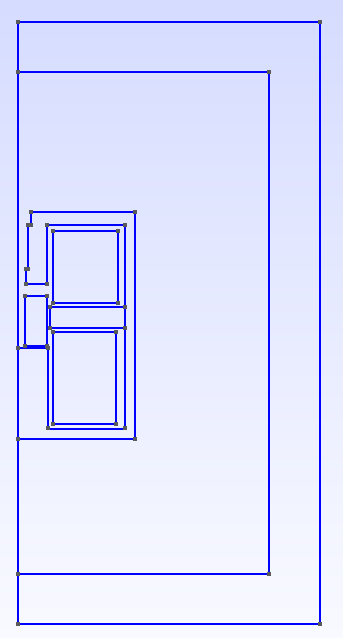
\includegraphics[width=0.35 \linewidth]{figures/model.png}
	\label{fig:model}
	}
	\hspace{0.16 \linewidth}
	\subfigure[Qt实现填充区域]{
	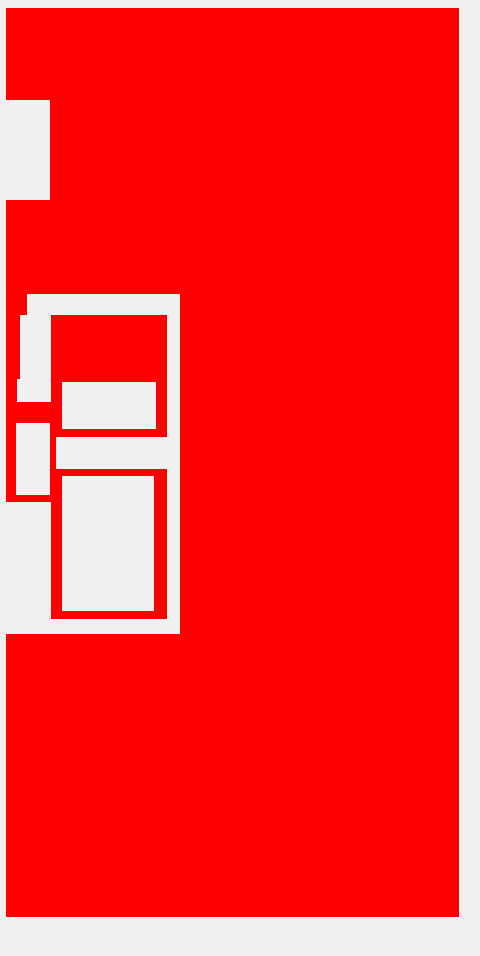
\includegraphics[width=0.33 \linewidth]{figures/path1.png}
	\label{fig:path1}
	}
	\caption{CAD模型以及空气区域的填充效果}
\end{figure}
然后令人比较惊奇的是,这个类还可以检测点是否在路径的内部,虽然并没有搞懂绘制路径的原理,但是莫名的好使,需要进一步研究路径的原理来使用它。

在填充路径时要用到填充规则,这里一共有两个填充规则

path.setFillRule(Qt::OddEvenFill);//奇偶填充规则

如果要判断一个点是否在图形中,可以从该点向图形外引一条水平线,如果该水平线与图形的交点人个数为奇数,那么该点在在图形中。

只填充在图形内的点

path.setFillRule(Qt::WindingFill); //非零弯曲规则

如果要判断一个点是否在图形中,可以从该点向图形外引一条水平线,如果该水平线与图形的边线相交,这个边线是顺时针绘制的,就记为1,是逆时针绘制的就记为-1,然后将所有数值相加,结果不为0,那么该点就在图形中。

QPainterPath判断点在内部的算法:

1.检查path是否为空,点是否在path的边界内;

2.根据path当中的元素进行迭代;

3.针对每一个path,按照上面的方法,做一条水平线,计算交点的个数,最后统计交点的总数,如果是奇偶填充规则的话,偶数就代表不在区域内部,不填充;奇数代表在区域内,填充;如果是windingfill,就判断曲线的逆时针和顺时针的方向,最后求和是不是0。

但是,具体填充的是否不会是这样判断的吧,如果是这样的话,计算量有点大啊。
\subsection{有一个问题}
在开发的过程当中,发现不管是要实现的函数,要规划的任务,都实在太多了,一不小心就不知道开发到什么地步了,什么功能有没有实现,实现到什么程度了,有没有被测试,有没有bug,好不好使。应当有那样的一个任务板,设定好要实现的计划和任务,明确规定功能的详细内容以及预计完成的日期。
\subsection{插件放哪里?}
插件的声明,应该放在mainwindow当中吗?从插件的功能来看,这就不属于主窗口的东西,而是独立于它的一部分,但是由于主窗口留出了访问其内部资源的接口,所以,也不必在mainwindow中实现。

但是,这是人家插件系统当中的版本。人家是通过一个插件管理器来载入了所有的插件,进而能够访问所有的资源和功能。反正怎样写都可以实现。如果是单独开发的话,写到main当中,这样集成度更高一些,因为这本来就是自己写的,而不是第三方,所以为什么不能放进去?可以的。但是,一定要注意初始化的顺序,有些插件是依赖于别的插件的,有先后顺序之分的,不然资源还没有被创建,后面的都JJ了。
\subsection{qDebug重定位}
我有一个大胆的想法,在调试的过程当中,总是要去看qtcreator的输出信息,窗口要切换来去非常的繁琐,要是直接能够把信息定位到我的log窗口,那么就不需要切换窗口了。之所以想定位debug,是因为不想改太多的代码。

仔细地查了一下资料,实现的原理很简单,就是重新实现一个qdebug,也就是定义一个新的宏命令吧。
\subsection{绘图的交互}
在绘图的时候,是设置为必须先绘制所有的点,然后再连接得到线段,最后再生成面。还是,可以随意的绘制。

第一种的好处就是,整个图形都是由最底层的点的坐标组成的,只要修改点的坐标,整个图形就可以相应地进行更新,而另外一种,就必须对每一个图形进行修改,因为它的坐标都是内部的,与其他的没有什么联系。
\subsection{生成面的算法}
刚开始比较好奇计算机是怎样实现不规则形状多边形的填充的,就搜索了一下奇偶填充算法,真的找到了很多资料,有很多的算法。看着看着就看到了一个主题,平面内封闭区间的识别,这个问题应该与生成面的算法类似吧?看到有人提出用计算图形学当中的一个漫水填充算法,这个名字真的好形象,在区域内找一个点,然后就开始递归式的开始填充,如果没有碰到边界,就不断地向前搜索,最后所有的区域都被填充了。但是效率实在太低了,每个点都要进行判断。

但是,还是不如直接设置方便啊。数据量小的话,还是手动设置吧!
\subsection{treemodel}
qmodelindex这个变量它所指向的东西可能会变,因为它的含义是某行某列,而模型当中可能会插入一些数据,导致它的行列数已经发生了改变。但是index当中不是保存了数据的真实指针了吗?
\subsection{图形选择}
选择的实体,是要单独的保存出来呢,还是要标记为“选中”状态就可以了?按道理讲,没必要那样做。选中状态的效果,是采用了不同的笔刷来实现的,只要跟正常画的不一样,就会给人以选中的状态,因为在单击鼠标的那一刻,图形颜色改变了,有反馈说明被选中了,因为只有选中了才会有改变啊。cad并没有在每一个形状的draw函数当中单独的进行选中的判断,而是放到了graphicview当中集中处理。这样的好处就是节省代码量。

绘制图形前需要判断:
\begin{enumerate}
	\item 是否存在;
	\item 是否可见;
	\item 是否在显示区域内;
	\item 设置笔刷;
	\item 是否被选中;
\end{enumerate}
\subsection{调试}
大型软件怎么调试?光是编译有时候可能都得十几分钟,有的甚至有几小时,几天的,这种情况还整个跑起来调试不太现实吧,应该都是单个模块调试吧。
\subsection{更新}
以谁为更新依据原理应该是谁先获得焦点。
\subsection{Type argument of Q_DECLARE_METATYPE(T*) must be fully defined}

\subsection{}